%% Faire première slide sur la structure charactéristique
%% La seconde montre la solution en vidéo
%% après on fait un overprint avec la comparaison MPM FEM FVM

\begin{frame}{One-dimensional elastic-plastic media: Characteristic wave structures \cite{Wang}}
  \centering
  \movie[height = 0.8\paperheight,width=.6\linewidth, showcontrols,poster,loop,autostart]{%\begin{tikzpicture}[scale=0.9]
  \draw[thick] (0,0) --(3,0)--(3,3)--(0,3)--(0,0);
  \foreach \x in {0.5,1.,...,2.5} 
  \draw(\x,-0.2)circle(0.2);
  \foreach \x in {0.25,0.75,...,2.75} 
  \draw(-0.2,\x)circle(0.2);
  \draw(0,-0.4)--(3.,-0.4);
  \draw(-.4,0)--(-.4,3);
  \fill [pattern=north east lines](0.0,-0.8)rectangle+(3,0.4);
  \fill [pattern=north east lines](-.8,0.)rectangle+(0.4,3);
  \draw[>=stealth,<->](0,3.1)--node[above=1pt]{\footnotesize $l=3 \: m$}(3,3.1);
  %\draw[>=stealth,<->](0.1,0)--node[right=1pt]{\footnotesize $a=1 \: m$}(0.1,1);
  % \foreach \x in {0.,0.25,...,1} 
  % \draw[>=stealth,<-] (-0.5,\x)--(0.,\x);
  % \node(a)at(-1.75,0.5){\footnotesize $\vect{v}=\matrice{v^d\\0 \\0}$}; 
  \node[right] (a) at(3.25,1.5){\footnotesize $\vect{v}(\vect{x},t=0)=\matrice{v^d\\0 \\0}$}; 
  \draw[>=stealth,->](-2.5,2)--(-1.5,2)node(a)[anchor=north]{\footnotesize $\vect{e}_1$};
  \draw[>=stealth,->](-2.5,2)--(-2.5,3)node(a)[anchor=south]{\footnotesize $\vect{e}_2$};
\end{tikzpicture}


%%% Local Variables:
%%% mode: latex
%%% TeX-master: "../../presentation"
%%% End:

      }{section4/animation/EP_planewave.mp4}
\end{frame}

\begin{frame}{One-dimensional elastic-plastic media: Characteristic wave structures \cite{Wang}}
  \vskip -15pt
  \begin{overprint}
    \onslide<1>
    % \metroset{block=fill}
    \begin{columns}
      \begin{column}{0.48\textwidth}
        \begin{block}{\footnotesize Purely elastic}
          \centering
          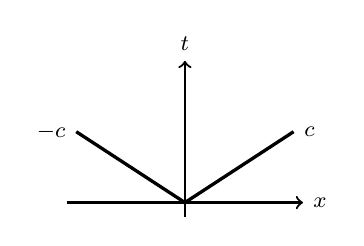
\begin{tikzpicture}[scale=0.6]
            \draw[thick,->] (-2.5,0) -- (2.5,0) node[right] {\footnotesize $x$};
            \draw[thick,->] (-0.,-0.3) -- (0,3) node[above] {\footnotesize $t$};
            \draw[very thick] (0,0) -- (2.3,1.5) node[right] {\footnotesize $c$};
            \draw[very thick] (0,0) -- (-2.3,1.5) node[left] {\footnotesize $-c$};
          \end{tikzpicture}
        \end{block}
      \end{column}
      \begin{column}{0.49\textwidth}
        \begin{block}{\footnotesize Plastic flow in the region $x>0$}
          \centering
          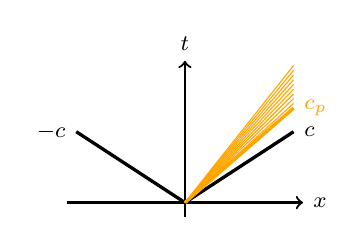
\begin{tikzpicture}[scale=0.6]
            \draw[thick,->] (-2.5,0) -- (2.5,0) node[right] {\footnotesize $x$};
            \draw[thick,->] (-0.,-0.3) -- (0,3) node[above] {\footnotesize $t$};
            \draw[very thick] (0,0) -- (2.3,1.5) node[right] {\footnotesize $c$};
            \draw[very thick] (0,0) -- (-2.3,1.5) node[left] {\footnotesize $-c$};
            \draw[very thick,Orange] (0,0) -- (2.3,2.) node[right] {\footnotesize $c_p$};
            \foreach \x in {0.,0.1,...,1.}
            \draw[Orange] (0,0.) -- (2.3,2.+\x);
          \end{tikzpicture}
        \end{block}
      \end{column}
    \end{columns}
    \footnotesize $c,c_p$: celerities of elastic and plastic waves

    \footnoteCite{Wang}
    
    \onslide<2>
      % \metroset{block=fill}
      \begin{columns}
        \begin{column}{0.48\textwidth}
          \begin{block}{\footnotesize Purely elastic}
            \centering
            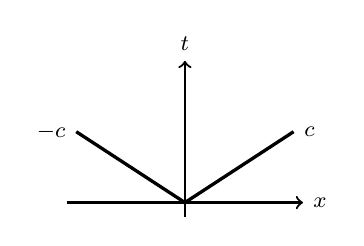
\begin{tikzpicture}[scale=0.6]
              \draw[thick,->] (-2.5,0) -- (2.5,0) node[right] {\footnotesize $x$};
              \draw[thick,->] (-0.,-0.3) -- (0,3) node[above] {\footnotesize $t$};
              \draw[very thick] (0,0) -- (2.3,1.5) node[right] {\footnotesize $c$};
              \draw[very thick] (0,0) -- (-2.3,1.5) node[left] {\footnotesize $-c$};
            \end{tikzpicture}
          \end{block}
        \end{column}
        \begin{column}{0.49\textwidth}
          \begin{block}{\footnotesize Plastic flow in the region $x>0$}
            \centering
            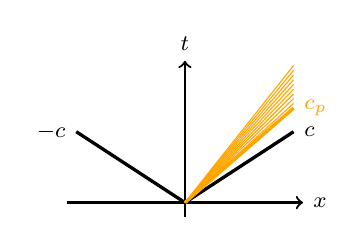
\begin{tikzpicture}[scale=0.6]
              \draw[thick,->] (-2.5,0) -- (2.5,0) node[right] {\footnotesize $x$};
              \draw[thick,->] (-0.,-0.3) -- (0,3) node[above] {\footnotesize $t$};
              \draw[very thick] (0,0) -- (2.3,1.5) node[right] {\footnotesize $c$};
              \draw[very thick] (0,0) -- (-2.3,1.5) node[left] {\footnotesize $-c$};
              \draw[very thick,Orange] (0,0) -- (2.3,2.) node[right] {\footnotesize $c_p$};
              \foreach \x in {0.,0.1,...,1.}
              \draw[Orange] (0,0.) -- (2.3,2.+\x);
            \end{tikzpicture}
          \end{block}
        \end{column}
      \end{columns}
      \begin{footnotesize}
        $c,c_p$: celerities of elastic and plastic waves
      \end{footnotesize}
      \metroset{block=fill}
      \begin{block}{\footnotesize Elastic-plastic Riemann solver \cite{Fogarty}}
        \footnotesize Account for \alert{plastic waves} by means of a prediction-correction approach
        \\ \alert{$\rightarrow$ use limiters for both elastic and plastic waves}
      \end{block}
      \footnoteCite{Wang,Fogarty}
  \end{overprint}
  
\end{frame}


\begin{frame}{}
  \begin{block}{Impact of one-dimensional elastic-plastic media \cite{Thomas_EP} (isotropic linear hardening)}
    Plane wave state:\: $\tens{\eps}=\eps \vect{e}_1 \otimes \vect{e}_1$ \quad ; \quad $\tens{\sigma}=\sigma \vect{e}_1\otimes \vect{e}_1 + \sigma_T\(\vect{e}_2\otimes \vect{e}_2+\vect{e}_3\otimes \vect{e}_3\)$
  \end{block}
  \begin{overprint}
    \onslide<1>
    \centering
    \input{section4/pgfFigures/ep_planeWave_stress_mpm_fem}

    \onslide<2>
    \centering
    \input{section4/pgfFigures/ep_planeWave_stress_dgmpm}
    
    \onslide<3>
    \centering
    \begin{tikzpicture}[scale=.7]
\begin{groupplot}[group style={group size=2 by 2,
ylabels at=edge left,horizontal sep=11.ex,
vertical sep=4ex,xticklabels at=edge bottom,xlabels at=edge bottom},
ymajorgrids=true,xmajorgrids=true,enlargelimits=0,xmin=0.,xmax=6.,xlabel=$x (m)$,
axis on top,scale only axis,width=0.48\linewidth,legend pos=outer north east
]
\nextgroupplot[title={\footnotesize Reflected waves -- Stress},ymin=-1.35e9,ymax=56579516.10614197,,xlabel=$x (m)$,ylabel=$\sigma \: (Pa)$]
\addplot[black,solid,mark=none,thick,mark size=3pt,mark repeat=2] coordinates{(0.0,-0.0) (0.12244897959183673,-0.0) (0.24489795918367346,-0.0) (0.36734693877551017,-0.0) (0.4897959183673469,-0.0) (0.6122448979591837,-700000000.0) (0.7346938775510203,-700000000.0) (0.8571428571428571,-700000000.0) (0.9795918367346939,-700000000.0) (1.1020408163265305,-1261004576.260559) (1.2244897959183674,-1261004576.260559) (1.346938775510204,-1261004576.260559) (1.4693877551020407,-1261004576.260559) (1.5918367346938775,-1261004576.260559) (1.7142857142857142,-1261004576.260559) (1.836734693877551,-1261004576.260559) (1.9591836734693877,-1261004576.260559) (2.0816326530612246,-1261004576.260559) (2.204081632653061,-1261004576.260559) (2.326530612244898,-1261004576.260559) (2.4489795918367347,-1261004576.260559) (2.571428571428571,-1261004576.260559) (2.693877551020408,-1261004576.260559) (2.816326530612245,-1261004576.260559) (2.9387755102040813,-1261004576.260559) (3.061224489795918,-1261004576.260559) (3.183673469387755,-1261004576.260559) (3.306122448979592,-1261004576.260559) (3.4285714285714284,-1261004576.260559) (3.5510204081632653,-1261004576.260559) (3.673469387755102,-1261004576.260559) (3.7959183673469385,-1261004576.260559) (3.9183673469387754,-1261004576.260559) (4.040816326530612,-1261004576.260559) (4.163265306122449,-1261004576.260559) (4.285714285714286,-1261004576.260559) (4.408163265306122,-1261004576.260559) (4.530612244897959,-1261004576.260559) (4.653061224489796,-1261004576.260559) (4.775510204081632,-1261004576.260559) (4.8979591836734695,-1261004576.260559) (5.020408163265306,-700000000.0) (5.142857142857142,-700000000.0) (5.26530612244898,-700000000.0) (5.387755102040816,-700000000.0) (5.5102040816326525,-0.0) (5.63265306122449,-0.0) (5.755102040816326,-0.0) (5.877551020408163,-0.0) (6.0,-0.0) };
\addplot[Red,dashed,mark=none,very thick,mark size=3pt,mark repeat=2] coordinates{(0.0,-8433215.03790355) (0.12244897959183673,-31379937.150059074) (0.24489795918367346,-73325965.87671247) (0.36734693877551017,-147815909.35881704) (0.4897959183673469,-264501011.32373637) (0.6122448979591837,-419797360.6339785) (0.7346938775510203,-586994803.1537646) (0.8571428571428571,-715242874.2277462) (0.9795918367346939,-804731796.1198385) (1.1020408163265305,-919403784.9173691) (1.2244897959183674,-1063504114.033879) (1.346938775510204,-1209904754.949398) (1.4693877551020407,-1304654513.0867395) (1.5918367346938775,-1291382612.5749428) (1.7142857142857142,-1218226204.6353252) (1.836734693877551,-1185455835.0777807) (1.9591836734693877,-1232745182.470082) (2.0816326530612246,-1261396271.0817113) (2.204081632653061,-1270103667.4391637) (2.326530612244898,-1227250869.598082) (2.4489795918367347,-1235273389.504192) (2.571428571428571,-1229787858.686364) (2.693877551020408,-1255621316.42765) (2.816326530612245,-1241442333.7811728) (2.9387755102040813,-1239848703.7218106) (3.061224489795918,-1239848703.7218091) (3.183673469387755,-1241442333.781176) (3.306122448979592,-1255621316.4276485) (3.4285714285714284,-1229787858.6863654) (3.5510204081632653,-1235273389.5041904) (3.673469387755102,-1227250869.598084) (3.7959183673469385,-1270103667.439164) (3.9183673469387754,-1261396271.081712) (4.040816326530612,-1232745182.4700806) (4.163265306122449,-1185455835.0777805) (4.285714285714286,-1218226204.6353254) (4.408163265306122,-1291382612.5749435) (4.530612244897959,-1304654513.0867395) (4.653061224489796,-1209904754.9493968) (4.775510204081632,-1063504114.033878) (4.8979591836734695,-919403784.917369) (5.020408163265306,-804731796.1198374) (5.142857142857142,-715242874.2277458) (5.26530612244898,-586994803.1537648) (5.387755102040816,-419797360.63397753) (5.5102040816326525,-264501011.3237358) (5.63265306122449,-147815909.35881624) (5.755102040816326,-73325965.8767119) (5.877551020408163,-31379937.150058918) (6.0,-8433215.037903389) };

\addplot[Orange,solid,mark=o,very thick,mark size=2pt,mark repeat=2] coordinates{(0.0,0.0) (0.12244897959183673,0.0) (0.24489795918367346,0.0) (0.36734693877551017,0.0) (0.4897959183673469,0.0) (0.6122448979591837,-700099961.461325) (0.7346938775510203,-702215400.6707044) (0.8571428571428571,-720845446.6905135) (0.9795918367346939,-807249777.2239016) (1.1020408163265305,-1021817726.088786) (1.2244897959183674,-1257135415.8766613) (1.346938775510204,-1201909815.2742617) (1.4693877551020407,-1284541316.0967622) (1.5918367346938775,-1197762497.5853782) (1.7142857142857142,-1280230396.1356874) (1.836734693877551,-1230639248.475009) (1.9591836734693877,-1232614670.2907715) (2.0816326530612246,-1296340561.1434355) (2.204081632653061,-1163180742.3691304) (2.326530612244898,-1344085453.2920678) (2.4489795918367347,-1125286993.986051) (2.571428571428571,-1354573027.5700727) (2.693877551020408,-1144440690.6862848) (2.816326530612245,-1331966839.3238678) (2.9387755102040813,-1234245710.8866477) (3.061224489795918,-1234245710.8866642) (3.183673469387755,-1331966839.3238637) (3.306122448979592,-1144440690.6862931) (3.4285714285714284,-1354573027.570076) (3.5510204081632653,-1125286993.9860492) (3.673469387755102,-1344085453.2920709) (3.7959183673469385,-1163180742.369132) (3.9183673469387754,-1296340561.143439) (4.040816326530612,-1232614670.2907667) (4.163265306122449,-1230639248.4750104) (4.285714285714286,-1280230396.1356888) (4.408163265306122,-1197762497.5853772) (4.530612244897959,-1284541316.0967634) (4.653061224489796,-1201909815.2742698) (4.775510204081632,-1257135415.8766532) (4.8979591836734695,-1021817726.0887933) (5.020408163265306,-807249777.2238963) (5.142857142857142,-720845446.6905184) (5.26530612244898,-702215400.6706979) (5.387755102040816,-700099961.4613259) (5.5102040816326525,0.0) (5.63265306122449,0.0) (5.755102040816326,0.0) (5.877551020408163,0.0) (6.0,0.0) };
\addplot[Blue,solid,mark=+,thick,mark size=3pt,mark repeat=2] coordinates{(0.0,-3.2561158711216654e-07) (0.12244897959183673,-6.54162606232603e-22) (0.24489795918367346,0.0) (0.36734693877551017,3.2561158711216643e-07) (0.4897959183673469,-4.884173806682499e-07) (0.6122448979591837,-710637837.2357953) (0.7346938775510203,-747893724.781927) (0.8571428571428571,-827829409.8631966) (0.9795918367346939,-936780409.853217) (1.1020408163265305,-1054073198.2499647) (1.2244897959183674,-1144128439.1849532) (1.346938775510204,-1207925723.6670742) (1.4693877551020407,-1232372577.7948787) (1.5918367346938775,-1254253728.274747) (1.7142857142857142,-1243570946.3490026) (1.836734693877551,-1268139963.2569304) (1.9591836734693877,-1248035262.8872383) (2.0816326530612246,-1268992337.693115) (2.204081632653061,-1251285653.8729925) (2.326530612244898,-1266352346.5241969) (2.4489795918367347,-1253527311.8706975) (2.571428571428571,-1264419055.233534) (2.693877551020408,-1255474245.0991223) (2.816326530612245,-1261578869.0693417) (2.9387755102040813,-1258168698.6750736) (3.061224489795918,-1258168698.6750731) (3.183673469387755,-1261578869.069342) (3.306122448979592,-1255474245.0991209) (3.4285714285714284,-1264419055.233534) (3.5510204081632653,-1253527311.870696) (3.673469387755102,-1266352346.5241973) (3.7959183673469385,-1251285653.8729923) (3.9183673469387754,-1268992337.6931143) (4.040816326530612,-1248035262.8872375) (4.163265306122449,-1268139963.2569308) (4.285714285714286,-1243570946.3490026) (4.408163265306122,-1254253728.2747467) (4.530612244897959,-1232372577.7948787) (4.653061224489796,-1207925723.6670735) (4.775510204081632,-1144128439.1849532) (4.8979591836734695,-1054073198.2499645) (5.020408163265306,-936780409.853217) (5.142857142857142,-827829409.8631967) (5.26530612244898,-747893724.7819276) (5.387755102040816,-710637837.2357956) (5.5102040816326525,-4.884173806682498e-07) (5.63265306122449,0.0) (5.755102040816326,-4.884173806682498e-07) (5.877551020408163,0.0) (6.0,-4.884173806682498e-07) };
\addplot[Purple,solid,mark=x,thick,mark size=3pt,mark repeat=2] coordinates{(0.0,0.0) (0.12244897959183673,0.0) (0.24489795918367346,0.0) (0.36734693877551017,0.0) (0.4897959183673469,0.0) (0.6122448979591837,-700149009.8511133) (0.7346938775510203,-702792255.866507) (0.8571428571428571,-725326867.326901) (0.9795918367346939,-850156660.8530495) (1.1020408163265305,-1109984935.9712873) (1.2244897959183674,-1250258832.4370122) (1.346938775510204,-1260471082.9558206) (1.4693877551020407,-1260981625.9873586) (1.5918367346938775,-1261003693.8957453) (1.7142857142857142,-1261004546.9659622) (1.836734693877551,-1261004575.4299965) (1.9591836734693877,-1261004576.2405941) (2.0816326530612246,-1261004576.260158) (2.204081632653061,-1261004576.2605524) (2.326530612244898,-1261004576.260559) (2.4489795918367347,-1261004576.260559) (2.571428571428571,-1261004576.260559) (2.693877551020408,-1261004576.260559) (2.816326530612245,-1261004576.2605588) (2.9387755102040813,-1261004576.2605588) (3.061224489795918,-1261004576.260559) (3.183673469387755,-1261004576.2605588) (3.306122448979592,-1261004576.2605588) (3.4285714285714284,-1261004576.2605588) (3.5510204081632653,-1261004576.2605588) (3.673469387755102,-1261004576.2605588) (3.7959183673469385,-1261004576.260553) (3.9183673469387754,-1261004576.2601585) (4.040816326530612,-1261004576.2405944) (4.163265306122449,-1261004575.4299967) (4.285714285714286,-1261004546.9659626) (4.408163265306122,-1261003693.895745) (4.530612244897959,-1260981625.987358) (4.653061224489796,-1260471082.955823) (4.775510204081632,-1250258832.4370096) (4.8979591836734695,-1109984935.971287) (5.020408163265306,-850156660.8530501) (5.142857142857142,-725326867.326901) (5.26530612244898,-702792255.866507) (5.387755102040816,-700149009.8511133) (5.5102040816326525,0.0) (5.63265306122449,0.0) (5.755102040816326,0.0) (5.877551020408163,0.0) (6.0,0.0) };


\nextgroupplot[title={\footnotesize Reflected waves -- Plastic strain},ymin=-0.0034,ymax=0.0,xlabel=$x \:(m)$,ylabel=$\eps^p$]
\addplot[black,solid,mark=none,thick,mark size=3pt,mark repeat=2] coordinates{(0.0,-0.0) (0.12244897959183673,-0.0) (0.24489795918367346,-0.0) (0.36734693877551017,-0.0) (0.4897959183673469,-0.0) (0.6122448979591837,-0.0) (0.7346938775510203,-0.0) (0.8571428571428571,-0.0) (0.9795918367346939,-0.0) (1.1020408163265305,-0.002030785796418313) (1.2244897959183674,-0.002030785796418313) (1.346938775510204,-0.002030785796418313) (1.4693877551020407,-0.002030785796418313) (1.5918367346938775,-0.002030785796418313) (1.7142857142857142,-0.002030785796418313) (1.836734693877551,-0.002030785796418313) (1.9591836734693877,-0.002030785796418313) (2.0816326530612246,-0.002030785796418313) (2.204081632653061,-0.002030785796418313) (2.326530612244898,-0.002030785796418313) (2.4489795918367347,-0.002030785796418313) (2.571428571428571,-0.002030785796418313) (2.693877551020408,-0.002030785796418313) (2.816326530612245,-0.002030785796418313) (2.9387755102040813,-0.002030785796418313) (3.061224489795918,-0.002030785796418313) (3.183673469387755,-0.002030785796418313) (3.306122448979592,-0.002030785796418313) (3.4285714285714284,-0.002030785796418313) (3.5510204081632653,-0.002030785796418313) (3.673469387755102,-0.002030785796418313) (3.7959183673469385,-0.002030785796418313) (3.9183673469387754,-0.002030785796418313) (4.040816326530612,-0.002030785796418313) (4.163265306122449,-0.002030785796418313) (4.285714285714286,-0.002030785796418313) (4.408163265306122,-0.002030785796418313) (4.530612244897959,-0.002030785796418313) (4.653061224489796,-0.002030785796418313) (4.775510204081632,-0.002030785796418313) (4.8979591836734695,-0.002030785796418313) (5.020408163265306,-0.0) (5.142857142857142,-0.0) (5.26530612244898,-0.0) (5.387755102040816,-0.0) (5.5102040816326525,-0.0) (5.63265306122449,-0.0) (5.755102040816326,-0.0) (5.877551020408163,-0.0) (6.0,-0.0) };
\addplot[Red,dashed,mark=none,very thick,mark size=3pt,mark repeat=2] coordinates{(0.0,0.0) (0.12244897959183673,0.0) (0.24489795918367346,0.0) (0.36734693877551017,0.0) (0.4897959183673469,0.0) (0.6122448979591837,0.0) (0.7346938775510203,0.0) (0.8571428571428571,-5.5177825258810104e-05) (0.9795918367346939,-0.0003791196239632164) (1.1020408163265305,-0.0007942218458547296) (1.2244897959183674,-0.0013158519965027296) (1.346938775510204,-0.0018458090676901286) (1.4693877551020407,-0.002188794617508559) (1.5918367346938775,-0.002229697455331896) (1.7142857142857142,-0.002258121963594508) (1.836734693877551,-0.002271799079674154) (1.9591836734693877,-0.002320613632318322) (2.0816326530612246,-0.002313868472160546) (2.204081632653061,-0.0024020122032007017) (2.326530612244898,-0.0023588630990294623) (2.4489795918367347,-0.0025433455597807667) (2.571428571428571,-0.002385435935351422) (2.693877551020408,-0.0027693350417516906) (2.816326530612245,-0.0024065265204776445) (2.9387755102040813,-0.0032250612006492966) (3.061224489795918,-0.0032250612006492524) (3.183673469387755,-0.002406526520477666) (3.306122448979592,-0.0027693350417516823) (3.4285714285714284,-0.0023854359353514295) (3.5510204081632653,-0.0025433455597807628) (3.673469387755102,-0.002358863099029464) (3.7959183673469385,-0.0024020122032006983) (3.9183673469387754,-0.0023138684721605448) (4.040816326530612,-0.002320613632318319) (4.163265306122449,-0.0022717990796741546) (4.285714285714286,-0.0022581219635945077) (4.408163265306122,-0.0022296974553318956) (4.530612244897959,-0.0021887946175085595) (4.653061224489796,-0.001845809067690125) (4.775510204081632,-0.0013158519965027254) (4.8979591836734695,-0.0007942218458547295) (5.020408163265306,-0.0003791196239632123) (5.142857142857142,-5.5177825258808404e-05) (5.26530612244898,0.0) (5.387755102040816,0.0) (5.5102040816326525,0.0) (5.63265306122449,0.0) (5.755102040816326,0.0) (5.877551020408163,0.0) (6.0,0.0) };

\addplot[Orange,solid,mark=o,very thick,mark size=2pt,mark repeat=2] coordinates{(0.0,0.0) (0.12244897959183673,0.0) (0.24489795918367346,0.0) (0.36734693877551017,0.0) (0.4897959183673469,0.0) (0.6122448979591837,-3.6185144371068533e-07) (0.7346938775510203,-8.019549939201378e-06) (0.8571428571428571,-7.545863055389513e-05) (0.9795918367346939,-0.00038823448768833166) (1.1020408163265305,-0.0011649510446652884) (1.2244897959183674,-0.0020167797859788647) (1.346938775510204,-0.002107399619958115) (1.4693877551020407,-0.002131770374563102) (1.5918367346938775,-0.0021403574192086572) (1.7142857142857142,-0.0021224712498380525) (1.836734693877551,-0.0021223153729543927) (1.9591836734693877,-0.002051517588290279) (2.0816326530612246,-0.00215869886386764) (2.204081632653061,-0.00229323761080671) (2.326530612244898,-0.002383730340592019) (2.4489795918367347,-0.002422023782426279) (2.571428571428571,-0.0024301527006305407) (2.693877551020408,-0.0023776240406298606) (2.816326530612245,-0.0022924966391795762) (2.9387755102040813,-0.002209718054457858) (3.061224489795918,-0.002209718054457853) (3.183673469387755,-0.00229249663917957) (3.306122448979592,-0.002377624040629834) (3.4285714285714284,-0.0024301527006305133) (3.5510204081632653,-0.0024220237824262893) (3.673469387755102,-0.0023837303405920274) (3.7959183673469385,-0.0022932376108067225) (3.9183673469387754,-0.002158698863867652) (4.040816326530612,-0.0020515175882902612) (4.163265306122449,-0.00212231537295439) (4.285714285714286,-0.002122471249838043) (4.408163265306122,-0.002140357419208655) (4.530612244897959,-0.0021317703745630944) (4.653061224489796,-0.0021073996199581038) (4.775510204081632,-0.002016779785978835) (4.8979591836734695,-0.0011649510446653149) (5.020408163265306,-0.00038823448768831226) (5.142857142857142,-7.54586305539126e-05) (5.26530612244898,-8.019549939178096e-06) (5.387755102040816,-3.6185144371335306e-07) (5.5102040816326525,0.0) (5.63265306122449,0.0) (5.755102040816326,0.0) (5.877551020408163,0.0) (6.0,0.0) };
\addplot[Blue,solid,mark=+,thick,mark size=3pt,mark repeat=2] coordinates{(0.0,0.0) (0.12244897959183673,0.0) (0.24489795918367346,0.0) (0.36734693877551017,0.0) (0.4897959183673469,0.0) (0.6122448979591837,-3.850800809337606e-05) (0.7346938775510203,-0.00017337094943683953) (0.8571428571428571,-0.00046273089543238553) (0.9795918367346939,-0.000857123655577256) (1.1020408163265305,-0.0012817129348415013) (1.2244897959183674,-0.0016077047572306) (1.346938775510204,-0.0018386451535459692) (1.4693877551020407,-0.0019271405531036338) (1.5918367346938775,-0.002006348337646142) (1.7142857142857142,-0.002018045326373221) (1.836734693877551,-0.002056615251608797) (1.9591836734693877,-0.0020613216365693464) (2.0816326530612246,-0.002064203896841495) (2.204081632653061,-0.0020644266901542695) (2.326530612244898,-0.0020621094945296272) (2.4489795918367347,-0.002062767607181189) (2.571428571428571,-0.002061489252343496) (2.693877551020408,-0.0020573197208032658) (2.816326530612245,-0.0020502799029179) (2.9387755102040813,-0.0020377776694292327) (3.061224489795918,-0.0020377776694292327) (3.183673469387755,-0.002050279902917899) (3.306122448979592,-0.002057319720803265) (3.4285714285714284,-0.0020614892523434956) (3.5510204081632653,-0.0020627676071811878) (3.673469387755102,-0.0020621094945296285) (3.7959183673469385,-0.0020644266901542695) (3.9183673469387754,-0.0020642038968414953) (4.040816326530612,-0.0020613216365693477) (4.163265306122449,-0.002056615251608799) (4.285714285714286,-0.0020180453263732205) (4.408163265306122,-0.0020063483376461405) (4.530612244897959,-0.0019271405531036334) (4.653061224489796,-0.0018386451535459673) (4.775510204081632,-0.0016077047572305996) (4.8979591836734695,-0.0012817129348415002) (5.020408163265306,-0.0008571236555772557) (5.142857142857142,-0.000462730895432386) (5.26530612244898,-0.0001733709494368422) (5.387755102040816,-3.850800809337776e-05) (5.5102040816326525,0.0) (5.63265306122449,0.0) (5.755102040816326,0.0) (5.877551020408163,0.0) (6.0,0.0) };
\addplot[Purple,solid,mark=x,thick,mark size=3pt,mark repeat=2] coordinates{(0.0,0.0) (0.12244897959183673,0.0) (0.24489795918367346,0.0) (0.36734693877551017,0.0) (0.4897959183673469,0.0) (0.6122448979591837,-5.394021759754931e-07) (0.7346938775510203,-1.010771354391672e-05) (0.8571428571428571,-9.168096769918878e-05) (0.9795918367346939,-0.0005435535234499527) (1.1020408163265305,-0.0014841083655069223) (1.2244897959183674,-0.001991887176242578) (1.346938775510204,-0.002028854598935097) (1.4693877551020407,-0.0020307027185062754) (1.5918367346938775,-0.002030782602337539) (1.7142857142857142,-0.0020307856903745234) (1.836734693877551,-0.002030785793411752) (1.9591836734693877,-0.002030785796346042) (2.0816326530612246,-0.002030785796416862) (2.204081632653061,-0.002030785796418289) (2.326530612244898,-0.0020307857964183135) (2.4489795918367347,-0.0020307857964183135) (2.571428571428571,-0.0020307857964183135) (2.693877551020408,-0.0020307857964183135) (2.816326530612245,-0.0020307857964183135) (2.9387755102040813,-0.0020307857964183135) (3.061224489795918,-0.0020307857964183135) (3.183673469387755,-0.0020307857964183135) (3.306122448979592,-0.0020307857964183126) (3.4285714285714284,-0.0020307857964183135) (3.5510204081632653,-0.0020307857964183126) (3.673469387755102,-0.0020307857964183126) (3.7959183673469385,-0.002030785796418291) (3.9183673469387754,-0.0020307857964168632) (4.040816326530612,-0.0020307857963460427) (4.163265306122449,-0.0020307857934117523) (4.285714285714286,-0.002030785690374525) (4.408163265306122,-0.0020307826023375384) (4.530612244897959,-0.0020307027185062733) (4.653061224489796,-0.002028854598935106) (4.775510204081632,-0.0019918871762425686) (4.8979591836734695,-0.0014841083655069208) (5.020408163265306,-0.0005435535234499549) (5.142857142857142,-9.168096769918878e-05) (5.26530612244898,-1.010771354391672e-05) (5.387755102040816,-5.394021759754931e-07) (5.5102040816326525,0.0) (5.63265306122449,0.0) (5.755102040816326,0.0) (5.877551020408163,0.0) (6.0,0.0) };

\addlegendentry{exact}
\addlegendentry{mpm -- CFL=0.5\color{white}0.5}
\addlegendentry{fem -- CFL=1}
\addlegendentry{dgmpm -- CFL=1}
\addlegendentry{fvm (SB) -- CFL=1}

\end{groupplot}
\end{tikzpicture}
%%% Local Variables:
%%% mode: latex
%%% TeX-master: "../../presentation"
%%% End:

      
  \end{overprint}
  \vspace{-0.1cm}
  \footnoteCite{Thomas_EP}
\end{frame}

%%%%%%


%%% Local Variables:
%%% mode: latex
%%% TeX-master: "../presentation"
%%% End: